\documentclass{note}
\usepackage{tikz}
\usetikzlibrary{positioning}
\tikzset{node/.style={draw,circle,scale=1.5}}
\title{HZOJ-72猜拳}
\author{宋星霖}
\date{\today}
\begin{document}
\maketitle
\section{题目描述}
\begin{leftbar}
\subsection{题目描述}
​在一次聚会中,每人拿着一张印有石头、剪刀、布的卡片,每个人具体拿得是哪种卡片不得而知。

​现在告诉你某些人之间的胜负关系,并会询问某两个人之间的对战结果,人按
照从$1$到$n$编号。

​对于每个询问,请给出正确的回答:\verb|Win(胜)、Loss(负)、Tie(平)|
\subsection{输入}
第一行输入两个整数$n,m(1 \leq n\leq10000,\quad
3\leq m \leq 10000)$

接下来m行,每行三个整数$a,\,b,\,c$
$\left( a \in \left[ 1, \, 2 \right], \: 1 \leq b,c\leq n\right)$
\begin{enumerate}
\item 当$a=1$时,代表新增一条已知信息,表示$b,\,c$对战中$b$胜
\item 当$a=2$时,代表根据以上信息,询问$b,\,c$对战中$b$​的结果
\end{enumerate}
如果出现某条新增的信息与之前的信息发生冲突,就忽略此条信息。
\subsection{输出}
对于每个$a=2$的操作,输出\verb|Win、Loss、Tie或Unknown|代表对战双方的结果。
\end{leftbar}
\section{算法解析}
对于这道题目,需要用到带权并查集。

\subsection{第1步:构建带权并查集}
带权并查集就是每一条边上面也有对应的数字。在这里,笔者与读者约定:
0代表Tie,1代表Loss,2代表Win。

带权并查集的实现方法也很简单。只需要多开一个val数组,表示第i个节点和父节点的结果。

对于这个题目,如果两个节点没有联通,就可以输出 \verb|Unknown| 。

\subsection{第2步:设计权值}
因为0代表Tie,1代表Loss,2代表Win,可以得到权值以3为周期重复结果。
所以,计算两个点的权值可以统计从A点走到B点的权值总和,再对3取余就是
A点到B点的权值。

因为A点到B点是2,B点到A点是1,又因为-2和1是同余数系,所以B点到A点也可以是-2。
类似的,如果A点到B点是1,B点到A点可以是-1。

所以,统计A点到B点权值总和的方法是:正着走加权值,倒着走减权值。

\subsection{第三步:设计合并方法}
对于下面的带权并查集,应该怎么合并呢?\\
\\
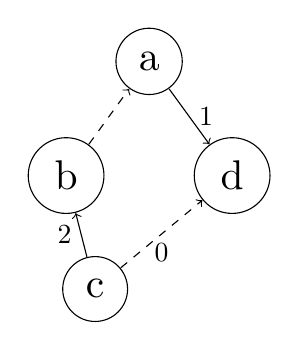
\begin{tikzpicture}
\node[node] (a) {a};
\node[node,below = 15pt of a,xshift = -20pt] (b) {b};
\node[node,below=15pt of b,xshift = 7pt] (c) {c};
\node[node,below=15pt of a,xshift = 20pt] (d) {d};
\path[<-] (b) edge node[left] {2} (c);
\path [->] (a) edge node[right] {1} (d);
\path[->,dashed] (c) edge node[below] {0} (d);
\path[->,dashed] (b) edge (a);
\end{tikzpicture}
\par
其实,b到a的权值是b到c,c到d,d到a的权值之和对3取余的值。也就是\\
$ -2 + 0 + 1 = -1 $。
不过,结果是负数,我们可以先加1个3,再取余。也就是 $ (-1 + 3) \mod 3 = 2 $。

\section{代码演示}
\begin{lstlisting}[style=C++,caption={HZOJ-72}]
#include <bits/stdc++.h>
using namespace std;
class UnionSet {
    public:
    UnionSet (int n) : fa (n + 1), code (n + 1, 0) {
        for (int i = 0; i <= n; i++) {
            fa[i] = i;
        }
    }
    int find (int x) {
        if (fa[x] == x)
        return x;
        int xx = find (fa[x]);
        code[x] = (code[x] + code[fa[x]] + 3) % 3;
        return fa[x] = xx;
    }
    void merge (int a, int b) {
        int aa = find (a), bb = find (b);
        if (aa == bb)
        return;
        code[aa] = (2 - code[a] + code[b] + 3) % 3;
        fa[aa] = bb;
    }
    vector<int> fa, code;
};
int main () {
    int n, m;
    scanf ("%d%d", &n, &m);
    UnionSet u (n);
    int a, b, c;
    for (int i = 0; i < m; i++) {
        scanf ("%d%d%d", &a, &b, &c);
        if (a == 1) {
            u.merge (b, c);
        } else {
            if (u.find (b) != u.find (c)) {
                printf ("Unknown\n");
                continue;
            }
            switch ((u.code[b] - u.code[c] + 3) % 3) {
                case 0:
                printf ("Tie\n");
                break;
                case 1:
                printf ("Loss\n");
                break;
                case 2:
                printf ("Win\n");
                break;
            }
        }
    }
    return 0;
}


\end{lstlisting}
\end{document}